\documentclass[twocolumn]{article}
\usepackage{authblk} 
\usepackage{graphicx} % Required for inserting images
\usepackage{subcaption}
\usepackage{amsmath} 
\usepackage{url} % for \url command
\usepackage{geometry}
\usepackage{float}

\geometry{
    top=1in,
    bottom=1in,
    left=0.5in,
    right=0.5in,
    columnsep=0.5in  % Adjust the column separation
}

\begin{document}
\title{\textbf{Physics Laboratory Report: Uniformly Accelerating Motion}}
\author{Your Name}
\affil{Instructor's Name:}
\affil{Group ID: X, Course \& Section Number: PHYSXXXX}
\date{Experiment Date: XXXX, Report Submission Date: XXXX}
\maketitle

\begin{abstract}
    This experiment investigates uniformly accelerating motion using a car and various sensors. The objective is to analyze the motion of the car under the influence of a constant force and compare the experimental results with theoretical predictions. The data collected includes the time taken by the car to travel between sensors placed at different distances.
\end{abstract}

\section{Introduction}
\label{sec:introduction}
Uniformly accelerating motion is a fundamental concept in physics, describing the motion of an object under constant acceleration. In this experiment, we study uniformly accelerating motion using a car on a track with sensors placed at regular intervals. By measuring the time taken by the car to travel between sensors, we can analyze its motion and compare the results with theoretical predictions.
\subsection{Objective}

The objective of this experiment is to investigate uniformly accelerating motion and compare the experimental results with the basic physical principles governing this type of motion.
\subsection{Basic Physical Principles}

The concept of uniformly accelerating motion can be understood by considering the following equations:

From Kinematics: 
\begin{equation}
v = v_0 + at
\label{eq:kinematics1}
\end{equation}

Using Equation~\ref{eq:kinematics1}, the following equations can be derived from \textit{Newton's Laws of Motion} for our experimental setup.

\begin{equation}
a=\frac{mg}{m+M }
\label{eq:a}
\end{equation}

\begin{equation}
v(t)=\frac{mg}{m+M}\cdot t
\label{eq:v_t_mass}
\end{equation}

\begin{equation}
x(t)=\frac{1}{2}\frac{mg}{m+M}\cdot t^{2}
\end{equation}

Considering a frictionless system, these equations describe the relationship between position, time, acceleration, and force in uniformly accelerating motion.

\section{Procedure}

The experiment began by setting up a track with sensors positioned at 15 cm, 30 cm, 45 cm, and 60 cm from the starting point. A car, attached to a string passing over a pulley, was used for the experiment. A mass of 10 g was attached to the car with the string to provide a constant force. The car was released, and the time taken for it to travel between each sensor was recorded. This process was repeated three times to obtain the mean time values for each sensor (see Table~\ref{tab:table2} from Section~\ref{sec:Results}). Velocities were calculated using the formula \(v = \frac{s}{t}\), where \(s\) is the distance and \(t\) is the time. Regression analysis was then performed on the data to establish the relationship between the variables.

\subsection{Setup}

The experimental setup consists of a car with a mass ($M$) of 390 g, a hanged mass ($m$) of 10 g, and sensors placed at 15 cm, 30 cm, 45 cm, and 60 cm from the start. The car is attached to a string passing over a pulley, with the hanged mass providing a constant force. The rails on which the car moves are constructed to have negligible friction, ensuring that the motion is primarily due to the applied force rather than frictional effects. This setup allows for the accurate measurement of the car's acceleration under the influence of the hanged mass. Each trial involves releasing the car from rest and recording the time taken for it to pass each sensor. 

Figure~\ref{fig:setup} and Figure~\ref{fig:setup_diagram} show the experiment setup used and the setup diagram for more clearance.
\begin{figure}[H]
    \begin{minipage}[t]{0.4\textwidth}
        \centering
        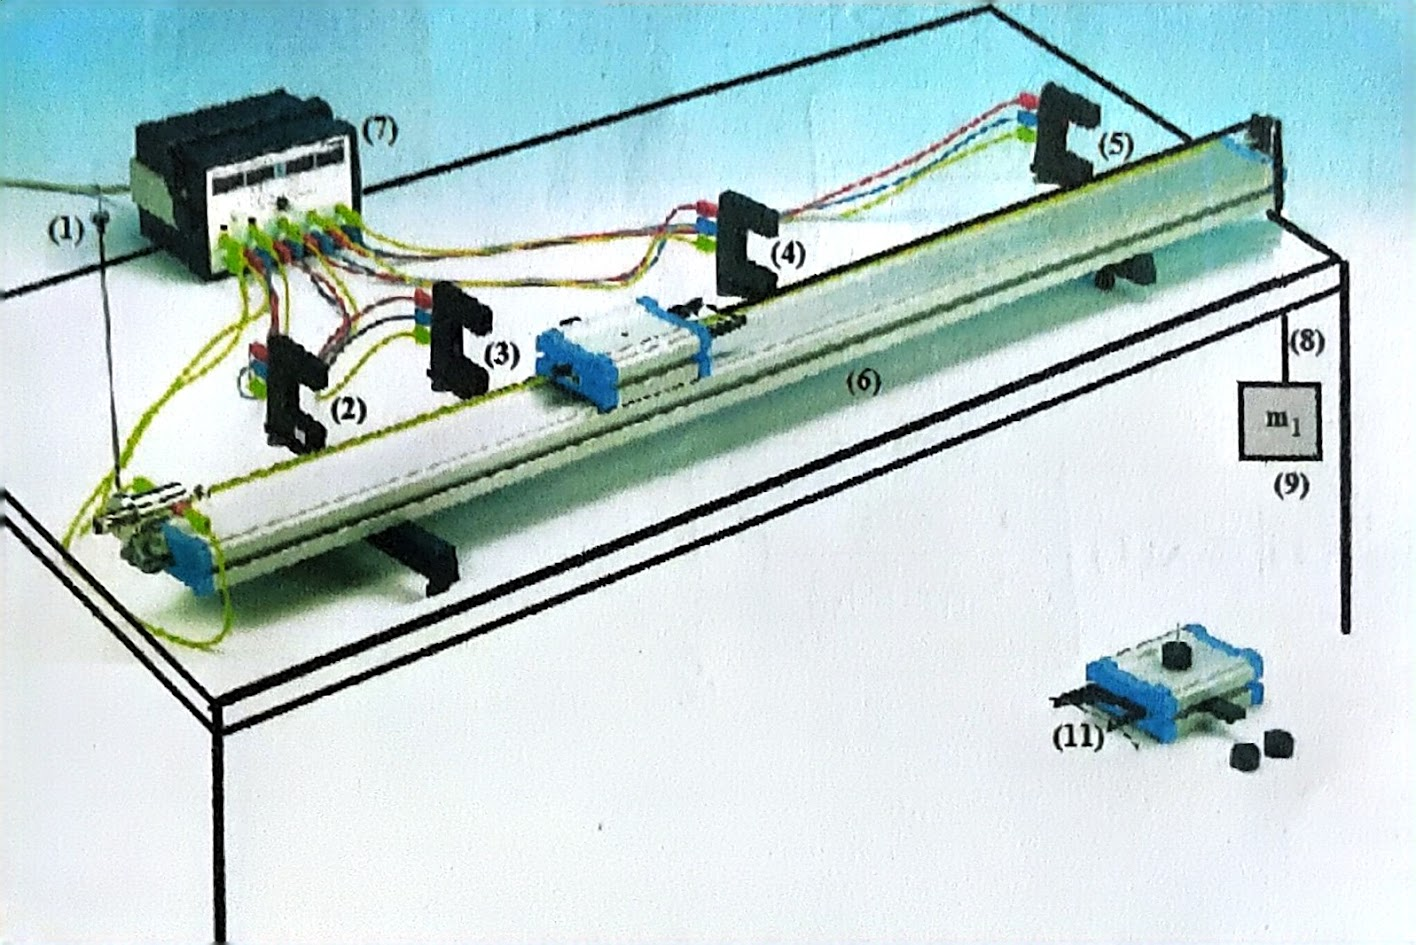
\includegraphics[width = 1 \textwidth]{setup.jpg}
        \caption{Uniformly Accelerating Motion Setup.}
        \label{fig:setup}
    \end{minipage}
    \hfill
    \begin{minipage}[t]{0.4\textwidth}
        \centering
        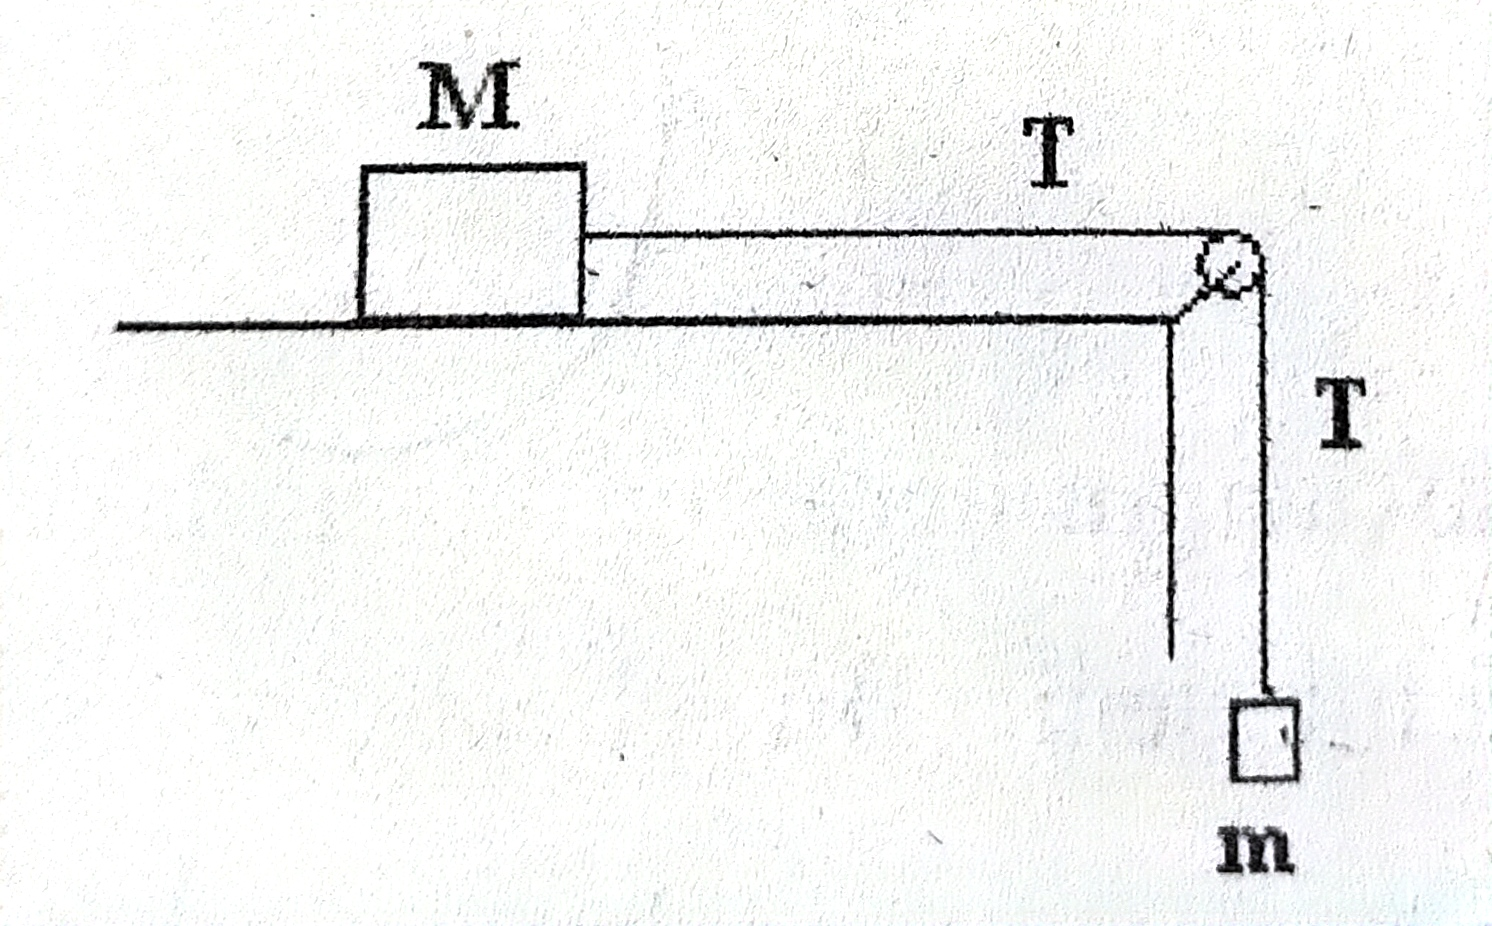
\includegraphics[width = 1 \textwidth]{setup_digram.jpg}
        \caption{Setup Diagram.}
        \label{fig:setup_diagram}
    \end{minipage}
\end{figure}
The sensors offer different modes of time measurement. One mode records the time \(t\) until the sensor detects the car's tip (Mode 1), while another measures the time interval \(\Delta t\) for the car to pass the sensor from its tip to its tail (Mode 2).

\subsection{Calculations}

Beside the Equations mentioned in Section~\ref{sec:introduction}, the time taken by the car when its center passes through the sensors is calculated by the following equation:
\begin{equation}
    t' = t_i + \frac{\Delta t_i}{2}
    \label{eq:t'}
\end{equation}
Equation~\ref{eq:t'} uses the time measured from the first and second modes of the sensors used.

\section{Results}
\label{sec:Results}

The results of the experiment are summarized in the following table:

\begin{table}[h]
    \centering
    \caption{Time data and calculated velocities used with Mode 1}
    \label{tab:table2}
    \begin{tabular}{cccc}
    \hline
    index & Position (m) & $t_i$ (s) & $v_i$ (m/s) \\
    \hline
    1 & 0.15 & 1.31 & 0.115 \\
    2 & 0.30 & 1.843 & 0.163 \\
    3 & 0.45 & 2.24 & 0.201 \\
    4 & 0.60 & 2.575 & 0.233 \\
    \hline
    \end{tabular}
\end{table}

\begin{figure}
    \centering
    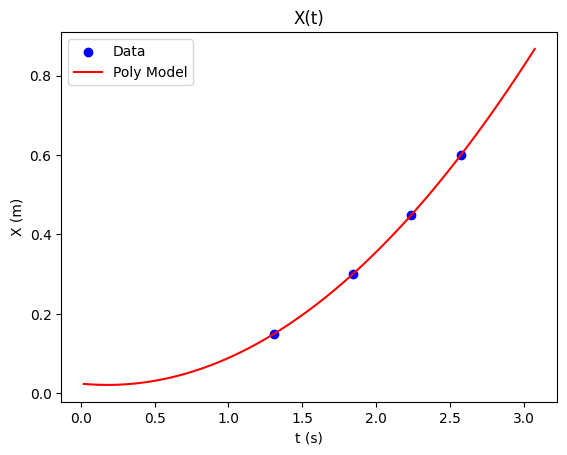
\includegraphics[width=0.5 \textwidth]{x(t).png}
    \caption{Gathered data and polynomial regression model is displayed for the $x(t)$ graph of Table~\ref{tab:table2}.}
    \label{fig:x(t)}
\end{figure}

\begin{figure}
    \centering
    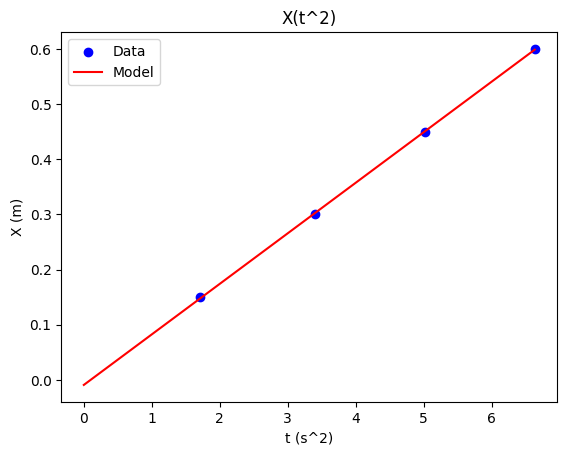
\includegraphics[width=0.5 \textwidth]{x(t^2).png}
    \caption{Gathered data and linear regression model is displayed for the $x(t^2)$ graph for Table~\ref{tab:table2} as in Figure~\ref{fig:x(t)}.}
    \label{fig:x(t^2)}
\end{figure}


\begin{figure}
    \centering
    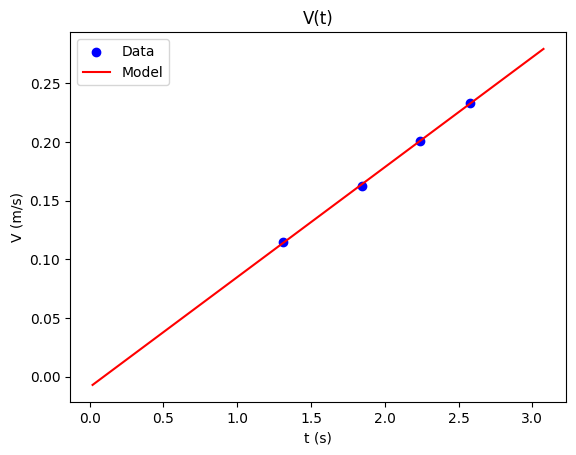
\includegraphics[width=0.5 \textwidth]{v(t).png}
    \caption{Calculated velocity data and time relation are displayed along with linear regression model.}
    \label{fig:V(t)}
\end{figure}


\begin{table}[H]
    \centering
    \caption{Raw data by Mode 2 used with the sensors. Where $t'$ and $v'$ are calculated 
    from Equations ~\ref{eq:t'} and ~\ref{eq:v_t_mass} respectively.}
    \label{tab:table3}
    \begin{tabular}{ccccc}
        \hline
        Trial & $\Delta t_1$ & $\Delta t_2$ & $\Delta t_3$& $\Delta t_4$ \\
        \hline
        1 & 0.368 & 0.276 & 0.230 &0.199\\
        2 & 0.369 & 0.278 & 0.233 &0.201\\
        3 & 0.374 & 0.281 & 0.234 &0.202\\
        \hline
        Mean & 0.370 & 0.278 & 0.232 & 0.201 \\
        \hline
        $t'$ & 1.494 & 1.983 & 2.356 & 2.671 \\
        \hline
        $v'$ & 0.366 & 0.486 & 0.577 & 0.656 \\
        \hline
            
    \end{tabular}
\end{table}


\begin{figure}
    \centering
    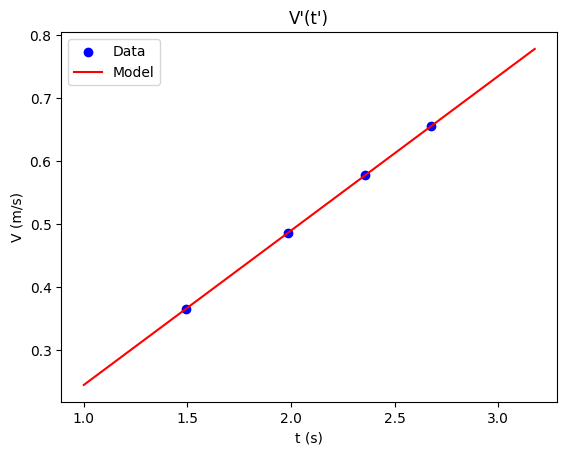
\includegraphics[width=0.5 \textwidth]{v'(t').png}
    \caption{Calculated $v'$ velocity data from Equation~\ref{eq:v_t_mass} and time relation are displayed along with linear regression model.}
    \label{fig:V'(t)}
\end{figure}

\begin{table}[H]
    \centering
    \caption{Data deliberately altering the car's mass ($m_2$) across measurements, alongside corresponding time readings ($t_4$) and distances from the fourth sensor ($x_4$).}
    \begin{tabular}{cccccc}
         \hline
         $m_1$ (gr) &  $m_2$ (gr) & $ m_1 + m_2$ (gr) & $t_4$ & $x_4$ & $a$ (m/s$^2$) \\
         \hline
          10 & 395 & 405 & 2.529  & 0.60 & 0.242\\
          10 & 400 & 410 & 2.546  & 0.60 & 0.239\\
          10 & 405 & 415 & 2.573  & 0.60 & 0.236\\
          10 & 410 & 420 & 2.667  & 0.60 & 0.233\\
    \end{tabular}
    \label{tab:m2_varying}
\end{table}

\begin{figure}
    \centering
    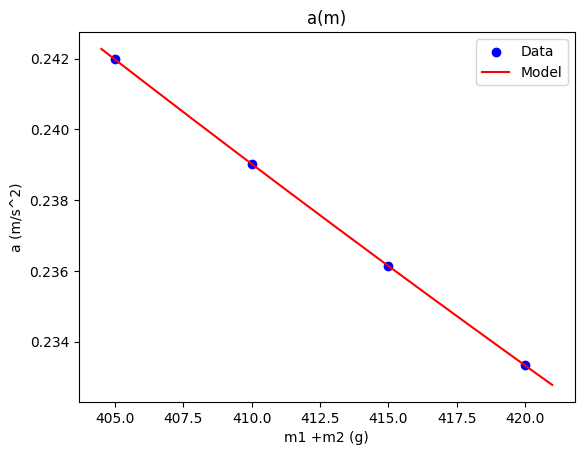
\includegraphics[width=0.5 \textwidth]{a(m).png}
    \caption{The table presents the calculated acceleration ($a$) data based on Equation~\ref{eq:a} and the mass relation for a constant force $F = m_1 g$, where m is denoted as $m_1$, and car's mas denoted as $m_2$, with $m_2$ varying as shown in Table~\ref{tab:m2_varying}. The table also includes a linear regression model for the data.}
    \label{fig:a(m)}
\end{figure}

\begin{table}[H]
    \centering
    \caption{}
    \begin{tabular}{cccccc}
         \hline
         $m_1$ (gr) &  $m_2'$ (gr) & $F=m_1g$ & $t_4$ & $x_4$ & $a$ (m/s$^2$) \\
         \hline
          14 & 396 & 137.2 & 2.107 & 0.60 & 0.00683 \\
          16 & 394 & 156.8 & 1.930 & 0.60 & 0.00780\\
          18 & 392 & 176.4 & 1.799 & 0.60 & 0.00878\\
          20 & 390 & 196.0 & 1.694 & 0.60 & 0.00976\\
    \end{tabular}
    \label{tab:F_varying}
\end{table}

\begin{figure}
    \centering
    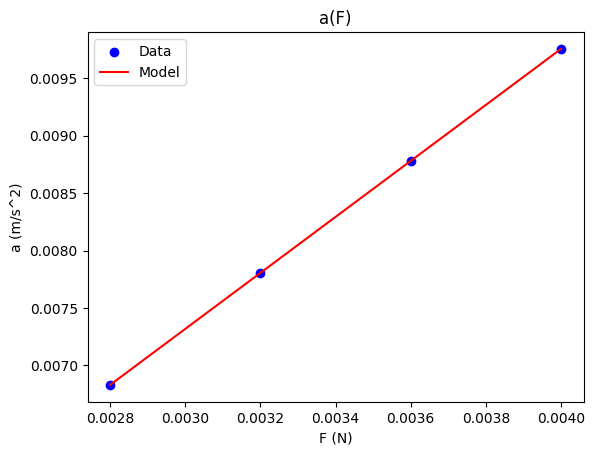
\includegraphics[width=0.5 \textwidth]{a(F).png}
    \caption{Calculated $a$ acceleration data from Equation~\ref{eq:a} and mass relation for a fixed $F$ force are displayed along with linear regression model where $m_1$ is $m$ and $m_2$ is $M$. $M$ here is the varing mass}
    \label{fig:a(F)}
\end{figure}


\section{Analysis and Discussion}
The experiment demonstrated the relationship between the applied force and the acceleration of the car, as well as the effect of the angle of inclination on the acceleration. The calculated acceleration due to gravity was close to the accepted value of \(9.81\) m/s\(^2\), indicating the accuracy of the experiment.

\section{Conclusion}
The experiment successfully investigated uniformly accelerating motion and provided insights into the principles of acceleration and gravity. The results were consistent with theoretical expectations, demonstrating the validity of the experiment.

\section{Additional Resources}
The following resources were used in conducting the experiment:
\begin{itemize}
    \item Physics textbook: "Fundamentals of Physics" by Halliday, Resnick, and Walker.
    \item Online resources: Physics classroom website (\url{www.physicsclassroom.com}).
\end{itemize}

\end{document}

\documentclass{article}
\usepackage{amsmath}
\usepackage{graphicx}
\usepackage{booktabs}

\title{Experimental Study of Uniformly Accelerating Motion}
\author{Your Name}
\date{\today}

\begin{document}

\maketitle

\begin{abstract}
    This experiment investigates uniformly accelerating motion using a car and various sensors. The objective is to analyze the motion of the car under the influence of a constant force and compare the experimental results with theoretical predictions. The data collected includes the time taken by the car to travel between sensors placed at different distances.
\end{abstract}

\section{Introduction}

Uniformly accelerating motion is a fundamental concept in physics, describing the motion of an object under constant acceleration. In this experiment, we study uniformly accelerating motion using a car on a track with sensors placed at regular intervals. By measuring the time taken by the car to travel between sensors, we can analyze its motion and compare the results with theoretical predictions.

\section{Experimental Setup}

The experimental setup consists of a car with a mass ($M_2$) of 390 g, a hanged mass ($m_1$) of 10 g, and sensors placed at 15 cm, 30 cm, 45 cm, and 60 cm from the start. The car is attached to a string passing over a pulley, with the hanged mass providing a constant force. The rails on which the car moves are constructed to have negligible friction, ensuring that the motion is primarily due to the applied force rather than frictional effects. This setup allows for the accurate measurement of the car's acceleration under the influence of the hanged mass. Each trial involves releasing the car from rest and recording the time taken for it to pass each sensor. Three trials are conducted to obtain a mean time value for each sensor, reducing the impact of any random errors in the timing measurements.


\section{Procedure}

The experiment began by setting up a track with sensors positioned at 15 cm, 30 cm, 45 cm, and 60 cm from the starting point. A car, attached to a string passing over a pulley, was used for the experiment. A hanged mass of 10 g was attached to the car to provide a constant force. The car was released, and the time taken for it to travel between each sensor was recorded. This process was repeated three times to obtain the mean time values for each sensor. Velocities were calculated using the formula \(V = \frac{s}{t}\), where \(s\) is the distance and \(t\) is the time. Linear regression analysis was then performed on the squared times and distances to establish the relationship between time squared and distance. Finally, a second-degree polynomial was fitted to the data to analyze the motion.

\section{Results}

The experimental results are summarized in Table \ref{tab:results} below.

\begin{table}[htbp]
    \centering
    \caption{Experimental Results}
    \label{tab:results}
    \begin{tabular}{cccc}
        \toprule
        Sensor Distance (m) & Mean Time (s) & Time Squared ($s^2$) & Velocity (m/s) \\
        \midrule
        0.15 & 1.309 & 1.715 & 0.115 \\
        0.30 & 1.843 & 3.399 & 0.163 \\
        0.45 & 2.240 & 5.017 & 0.201 \\
        0.60 & 2.575 & 6.632 & 0.233 \\
        \bottomrule
    \end{tabular}
\end{table}

The relationship between time squared and distance is shown in Figure \ref{fig:regression}.

\begin{figure}[htbp]
    \centering
    \includegraphics[width=0.6\textwidth]{regression.png}
    \caption{Regression Analysis of Time Squared vs. Distance}
    \label{fig:regression}
\end{figure}

The linear regression model for $t^2$ and $s$ is given by the equation:

\begin{equation}
    s = 0.0622t^2 - 0.0293
    \label{eq:linear}
\end{equation}

The polynomial regression model for the mean time values and distances is given by the equation:

\begin{equation}
    s = 0.013t^2 - 0.024t + 0.168
    \label{eq:polynomial}
\end{equation}

\section{Conclusion}

The experiment demonstrates the principles of uniformly accelerating motion and provides valuable insights into the relationship between time squared and distance. The results closely match the theoretical predictions, confirming the validity of the laws of motion.

\end{document}
